\documentclass[12pt]{article}
\usepackage[utf8]{inputenc}
\usepackage[english,russian]{babel}
\usepackage{graphicx}
\usepackage{amsmath}
\usepackage[a4paper,left=5mm,right=10mm,top=5mm,bottom=5mm]{geometry}

\DeclareMathSymbol{*}{\mathbin}{symbols}{"01}

\title{Title}
\author{Марк Вавилов}
\date{March 22 2023}

\begin{document}

\maketitle

\begin{tabular} { c | c | c | c | c | c }
1 & 2 & 3 & 4 & 5 & 6 \\ 
\hline
а & б & в &  &  &  \\ 
\hline
a & b & c &  &  &  \\ 
\hline
$x=40$ & $\implies $ & $\sqrt{\dfrac{(3.9*10^5)^2}{2*3.9*10^5}}$ &  &  &  \\
\end{tabular}

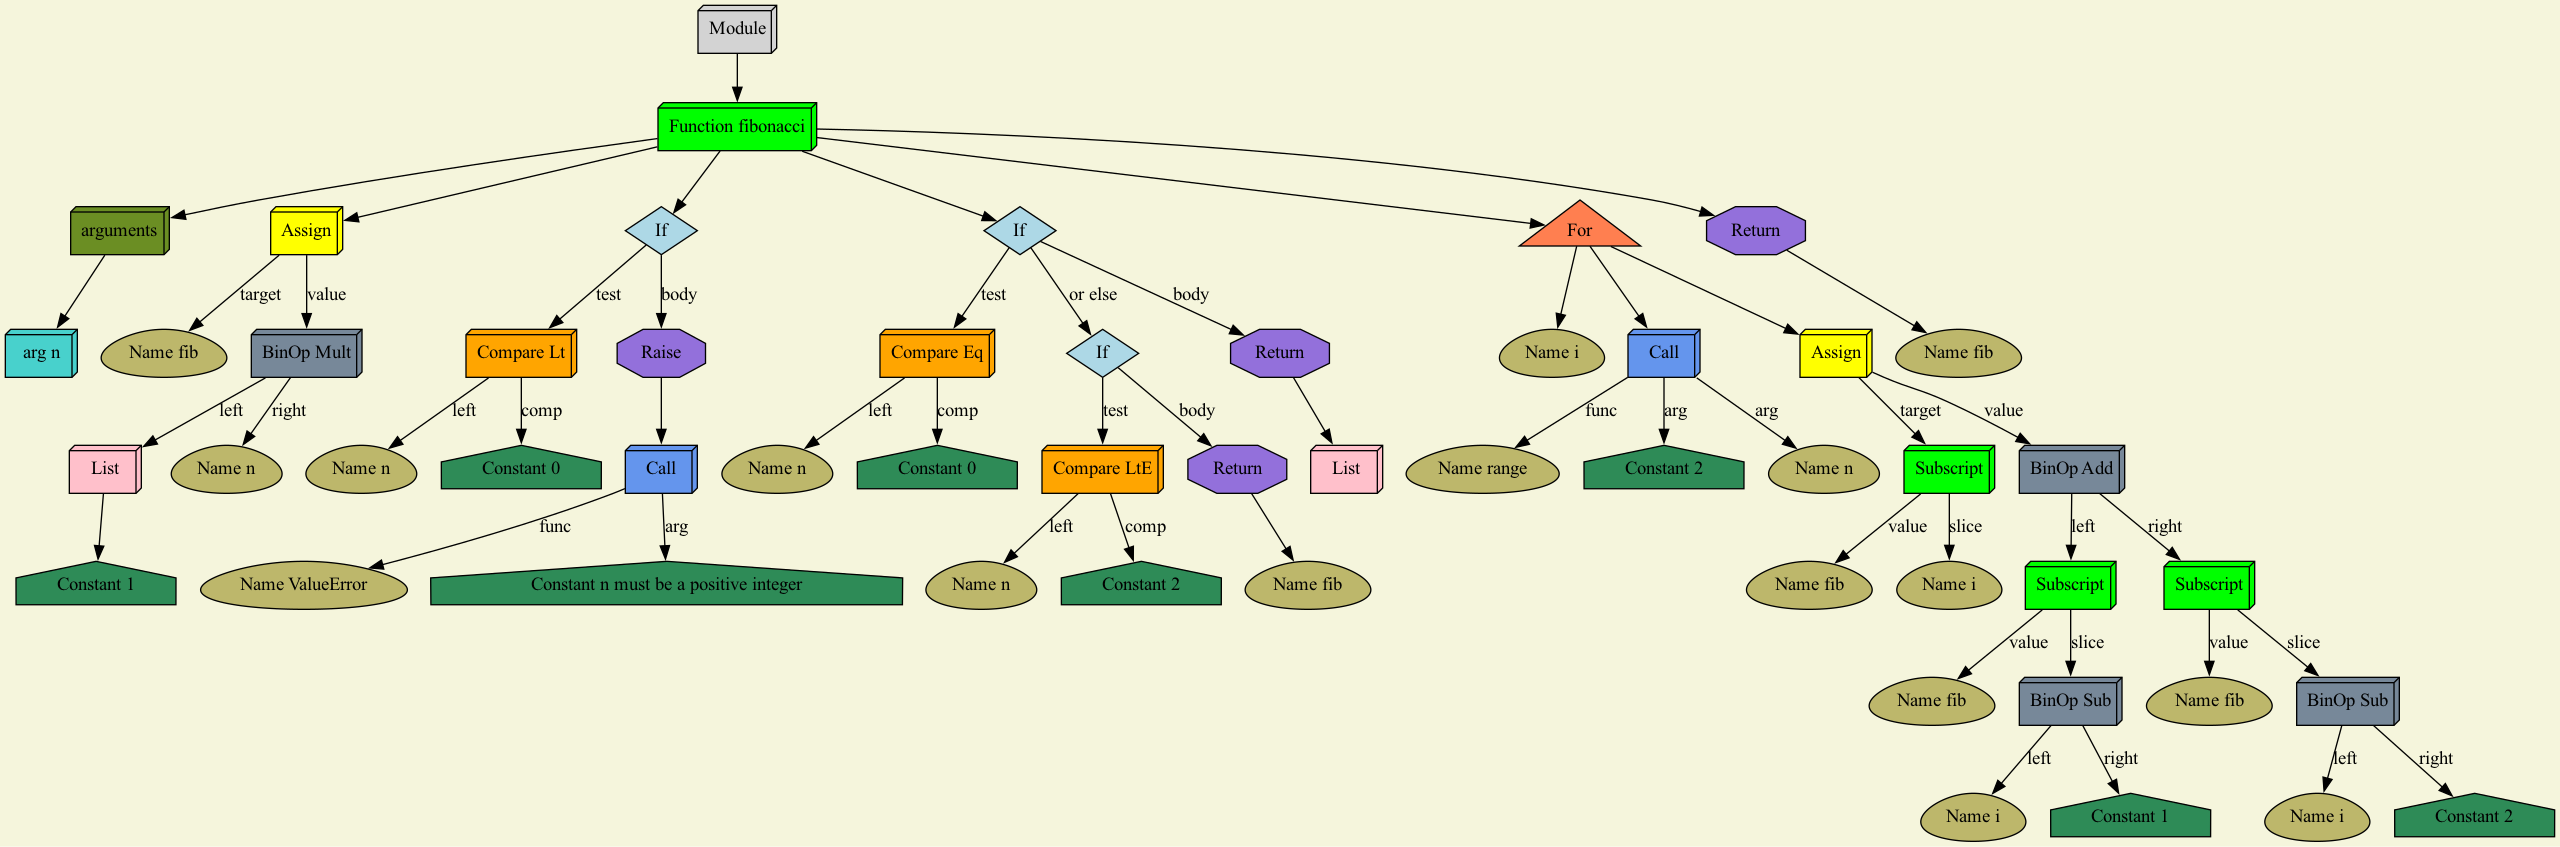
\includegraphics[scale=0.2]{../artifacts/graph.png}\\

\end{document}